\chapter{Analisi del Contesto}

\section{Descrizione del Contesto}

Il progetto si colloca nel mercato dell'\textbf{automotive post-vendita} e, in particolare, nell'ambito della personalizzazione dei veicoli, un comparto che negli ultimi anni ha acquisito una rilevanza economica crescente. Le modifiche apportate a un'automobile dopo l'immatricolazione --- interventi sulla meccanica, sull'assetto, sull'impianto frenante, sulla componentistica elettronica o sull'estetica --- non costituiscono più un fenomeno di nicchia, ma un segmento strutturato che coinvolge officine specializzate, produttori di componenti, concessionarie, enti di omologazione e compagnie assicurative.

A questa crescita non ha però corrisposto un'evoluzione degli strumenti di documentazione. Il ciclo di vita di un veicolo modificato continua a essere tracciato attraverso fatture, dichiarazioni di conformità, schede tecniche e annotazioni sul libretto di circolazione: strumenti eterogenei, prodotti da soggetti diversi, conservati su supporti non omogenei e privi di qualunque garanzia di integrità nel tempo. Ne deriva una \textbf{frammentazione documentale} che rende difficile, e in alcuni casi impossibile, ricostruire in modo affidabile che cosa sia stato realmente fatto su un determinato mezzo, da chi, con quali componenti e nel rispetto di quali requisiti.

\subsection*{Criticit\`a della filiera}

Le principali problematiche che caratterizzano il contesto possono essere ricondotte ai seguenti punti:

\begin{enumerate}
    \item \textbf{Asimmetria informativa}: il proprietario del veicolo, e a maggior ragione un potenziale acquirente, non dispone di alcuno strumento indipendente per verificare la natura e la provenienza delle modifiche effettuate. La documentazione \`e nella disponibilit\`a di chi ha eseguito l'intervento e la sua completezza dipende dalla diligenza del singolo operatore.

    \item \textbf{Vulnerabilit\`a della documentazione}: certificati e schede tecniche in formato cartaceo o digitale non protetto sono esposti a smarrimento, alterazione e falsificazione. La possibilit\`a di retrodatare un intervento o di sostituire una dichiarazione di conformit\`a non \`e tecnicamente impedita da alcun meccanismo.

    \item \textbf{Difficolt\`a di verifica della conformit\`a}: gli enti preposti al controllo e all'omologazione devono ricostruire manualmente la storia degli interventi prima di poter esprimere una valutazione. Ci\`o allunga i tempi delle procedure autorizzative e ne aumenta il costo, sia per l'ente sia per il cittadino.

    \item \textbf{Rischio di componenti non conformi}: l'assenza di tracciabilit\`a lungo la filiera dei ricambi rende difficile accertare che i pezzi installati siano originali e omologati, esponendo il veicolo a rischi di sicurezza e favorendo la diffusione di componentistica contraffatta.

    \item \textbf{Opacit\`a per il comparto assicurativo}: le compagnie non dispongono di informazioni attendibili sulle modifiche apportate al mezzo. Ne conseguono una stima imprecisa del rischio in fase di sottoscrizione, tempi di istruttoria pi\`u lunghi in caso di sinistro e una maggiore esposizione a dichiarazioni incomplete o mendaci.

    \item \textbf{Perdita di valore alla rivendita}: il proprietario che abbia investito in personalizzazioni eseguite a regola d'arte non \`e in grado di dimostrarne la qualit\`a e la regolarit\`a. L'incertezza si traduce in una svalutazione del mezzo sul mercato dell'usato.
\end{enumerate}

Si tratta, come si osserva, di criticit\`a che non colpiscono un singolo attore, ma che si distribuiscono lungo l'intera filiera e che hanno una radice comune: l'assenza di una \textbf{fonte informativa unica, condivisa e non alterabile} sullo stato del veicolo.

\subsection*{Il ruolo della tecnologia blockchain}

\`E su questo punto che si innesta l'idea progettuale. La tecnologia \textbf{blockchain}, intesa come registro distribuito (\textit{Distributed Ledger Technology}), risponde in modo nativo al problema individuato: consente di registrare informazioni in modo immutabile e verificabile da parte di pi\`u soggetti, senza che alcuno di essi possa alterare unilateralmente quanto gi\`a scritto e senza richiedere la presenza di un'autorit\`a centrale depositaria del dato.

Nel contesto in esame, l'adozione di un registro condiviso permette di trasformare la documentazione delle modifiche da insieme di documenti sparsi a \textbf{storico certificato} associato in modo univoco al veicolo. Ogni attore della filiera contribuisce al registro per la parte di propria competenza --- l'officina per le lavorazioni eseguite, il fornitore per la provenienza dei componenti, l'ente certificatore per l'esito delle verifiche --- e ciascuno pu\`o consultare, nei limiti delle proprie autorizzazioni, quanto registrato dagli altri.

Va tuttavia osservato che l'apertura informativa introdotta dal registro distribuito entra in tensione con un'esigenza altrettanto legittima, quella di \textbf{riservatezza} dei dati personali del proprietario e dei dati sensibili del veicolo. Come si vedr\`a nella modellazione che segue, tale tensione costituisce uno dei principali \textit{trade-off} progettuali del sistema e va governata attraverso politiche di accesso selettivo, piuttosto che risolta a favore dell'uno o dell'altro obiettivo.

\section{Modellazione del Contesto in GOREM}

Per rappresentare formalmente l'ecosistema in cui il progetto si inserisce si \`e adottata la metodologia \textbf{GOREM} (\textit{Goal-Oriented Requirement Engineering Methodology}). La modellazione del contesto costituisce lo strumento propedeutico alla definizione dei requisiti e alla successiva progettazione della piattaforma: essa individua i soggetti coinvolti, le qualit\`a che ciascuno di essi si attende dal sistema e le relazioni di rinforzo o di conflitto che intercorrono tra tali qualit\`a.

In questa fase l'analisi mantiene deliberatamente un respiro ampio, includendo anche attori che non interagiranno direttamente con la piattaforma. La restrizione a uno scenario specifico, con l'individuazione dei soli soggetti che operano sul sistema e dei ruoli da essi assunti, sar\`a oggetto del Capitolo~3.

\subsection{Stakeholder Diagram}

Il \textbf{Stakeholder Diagram} riportato in Figura~\ref{fig:stakeholder-diagram} identifica tutti i soggetti che, a vario titolo, gravitano attorno al mondo della personalizzazione dei veicoli. Gli attori sono raggruppati in sei categorie generali secondo la \textbf{funzione che svolgono all'interno della filiera}. Accanto a esse compare l'\textit{Intermediario}, che fornisce e gestisce la piattaforma: opera trasversalmente rispetto alla filiera ed \`e pertanto collegato direttamente alla radice della gerarchia.

\begin{figure}[H]
    \centering
    \makebox[\textwidth][c]{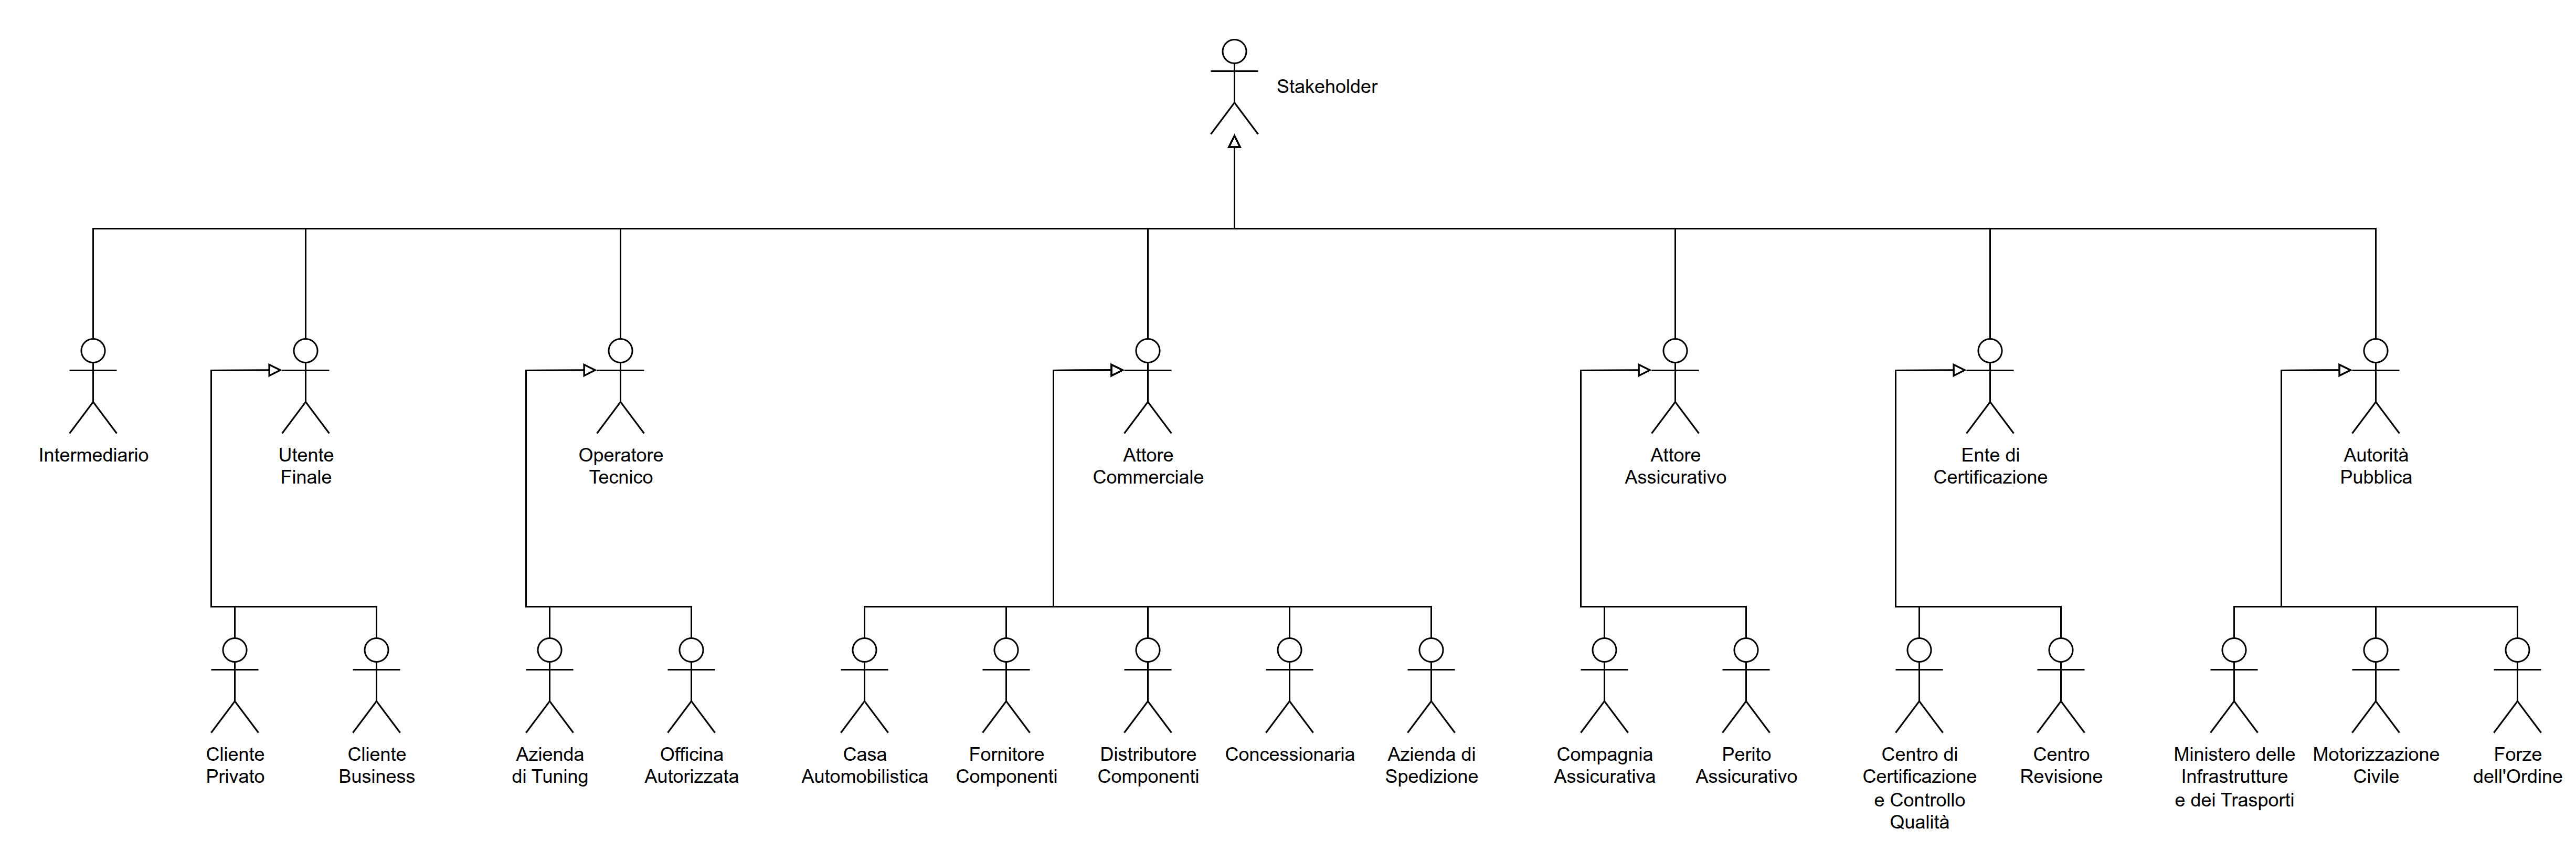
\includegraphics[width=1.3\textwidth]{imgs/context/stakeholders_diagram.png}}
    \caption{Stakeholder Diagram}
    \label{fig:stakeholder-diagram}
\end{figure}

Le categorie individuate, con i relativi attori specifici, sono le seguenti:

\begin{itemize}
    \item \textbf{Utente Finale}: raccoglie i soggetti che utilizzano il veicolo e ne subiscono direttamente le conseguenze in termini di sicurezza, valore e regolarit\`a amministrativa.
    \begin{itemize}
        \item \textit{Cliente Privato}: \`e l'utente finale che acquista il veicolo e commissiona le modifiche. Il suo interesse primario risiede nel disporre di un mezzo personalizzato, legalmente conforme e dotato di uno storico verificabile che ne tuteli il valore nel tempo.
        \item \textit{Cliente Business}: comprende le imprese e i gestori di flotte che impiegano veicoli commerciali allestiti o personalizzati. \`E interessato a dimostrare la conformit\`a dell'intero parco mezzi e a preservarne il valore residuo in sede di dismissione.
    \end{itemize}

    \item \textbf{Operatore Tecnico}: comprende i soggetti che intervengono materialmente sul veicolo.
    \begin{itemize}
        \item \textit{Azienda di Tuning}: esegue le modifiche funzionali ed estetiche commissionate. \`E interessata a valorizzare la qualit\`a del proprio operato e a tutelarsi da contestazioni infondate.
        \item \textit{Officina Autorizzata}: effettua interventi di manutenzione e installazione nel rispetto degli standard del costruttore. \`E interessata a dimostrare la conformit\`a delle lavorazioni eseguite.
    \end{itemize}

    \item \textbf{Attore Commerciale}: riunisce i soggetti che operano lungo la catena di fornitura e di distribuzione del veicolo e dei suoi componenti.
    \begin{itemize}
        \item \textit{Casa Automobilistica}: produce il veicolo base e ne detiene i dati ufficiali. \`E interessata alla tutela del marchio e al monitoraggio dell'impatto delle modifiche post-vendita sui propri mezzi.
        \item \textit{Fornitore Componenti}: produce la componentistica destinata alle modifiche ed \`e interessato ad attestare l'originalit\`a e le specifiche tecniche dei propri prodotti.
        \item \textit{Distributore Componenti}: cura la distribuzione dei ricambi verso officine e aziende di tuning, con interesse a dimostrare la tracciabilit\`a della merce trattata.
        \item \textit{Concessionaria}: rappresenta il punto di contatto commerciale con il cliente ed \`e interessata a offrire un servizio a valore aggiunto riducendo al contempo il rischio legale connesso alla vendita di veicoli modificati.
        \item \textit{Azienda di Spedizione}: cura la logistica di trasferimento del veicolo e della componentistica tra i diversi operatori della filiera, con interesse a documentare in modo incontestabile la presa in carico e la riconsegna del mezzo.
    \end{itemize}

    \item \textbf{Attore Assicurativo}: include i soggetti che assumono e valutano il rischio connesso alla circolazione del veicolo.
    \begin{itemize}
        \item \textit{Compagnia Assicurativa}: \`e interessata a disporre di informazioni attendibili sulle modifiche apportate, sia per una corretta valutazione del rischio in fase di sottoscrizione, sia per una gestione pi\`u rapida e oggettiva dei sinistri.
        \item \textit{Perito Assicurativo}: professionista incaricato di accertare lo stato del veicolo e l'entit\`a del danno in caso di sinistro. \`E interessato a ricostruire in modo rapido e attendibile la configurazione effettiva del mezzo al momento dell'evento.
    \end{itemize}

    \item \textbf{Ente di Certificazione}: raccoglie gli organismi terzi e accreditati che eseguono materialmente le verifiche tecniche sul veicolo e ne attestano la conformit\`a, rispondendo in proprio della correttezza del giudizio espresso. Il valore della loro attivit\`a dipende dal riconoscimento di cui gode il rispettivo accreditamento.
    \begin{itemize}
        \item \textit{Centro di Certificazione e Controllo Qualit\`a}: organismo terzo e imparziale che verifica la conformit\`a tecnica e normativa degli interventi, rilasciando la relativa certificazione. \`E l'unico soggetto della categoria che, nello scenario specifico definito nel Capitolo~3, opera direttamente sulla piattaforma.
        \item \textit{Centro Revisione}: esegue le verifiche periodiche obbligatorie ed \`e interessato a disporre di uno storico affidabile degli interventi subiti dal mezzo.
    \end{itemize}

    \item \textbf{Autorit\`a Pubblica}: comprende i soggetti titolari di potest\`a normativa e di vigilanza, cui competono la definizione delle regole tecniche, il riconoscimento formale delle modifiche e il controllo sulla sicurezza dei veicoli circolanti.
    \begin{itemize}
        \item \textit{Ministero delle Infrastrutture e dei Trasporti}: definisce il quadro normativo di riferimento in materia di omologazione e circolazione.
        \item \textit{Motorizzazione Civile}: \`e competente per l'aggiornamento della carta di circolazione e per il riconoscimento formale delle modifiche apportate.
        \item \textit{Forze dell'Ordine}: effettuano i controlli su strada ed \`e loro interesse poter verificare rapidamente la corrispondenza tra il veicolo e quanto risulta documentato.
    \end{itemize}
\end{itemize}

L'\textbf{Intermediario} \`e un soggetto specializzato nella gestione di piattaforme di tracciamento basate su DLT: fornisce l'infrastruttura tecnologica e funge da punto di contatto tecnico per tutti gli altri attori della filiera. Il suo interesse risiede nell'adozione della soluzione lungo l'intera catena del valore e nella sostenibilit\`a economica dell'esercizio, obiettivi che trovano espressione nei softgoal illustrati nel paragrafo seguente.

\subsection{Softgoal Diagram}

I \textbf{softgoal} rappresentano gli obiettivi non funzionali del sistema, ossia le qualit\`a che esso deve possedere per risultare accettabile e di successo agli occhi degli attori coinvolti. A differenza dei goal, essi non ammettono una verifica binaria di soddisfacimento, ma vengono perseguiti secondo un criterio di sufficienza.

Il diagramma riportato in Figura~\ref{fig:softgoal-diagram} \`e organizzato attorno a un softgoal radice, \textbf{Certificazione digitale affidabile delle modifiche ai veicoli}, che sintetizza la finalit\`a complessiva del sistema: garantire un ecosistema digitale sicuro e condiviso per la registrazione e la certificazione delle modifiche post-vendita dei veicoli attraverso l'utilizzo della tecnologia blockchain. A tale obiettivo generale concorrono trentacinque softgoal specifici, cinque per ciascuna delle sei categorie individuate e cinque propri dell'Intermediario; le linee continue collegano ogni softgoal allo stakeholder che ne \`e portatore.

\begin{figure}[H]
    \centering
    \makebox[\textwidth][c]{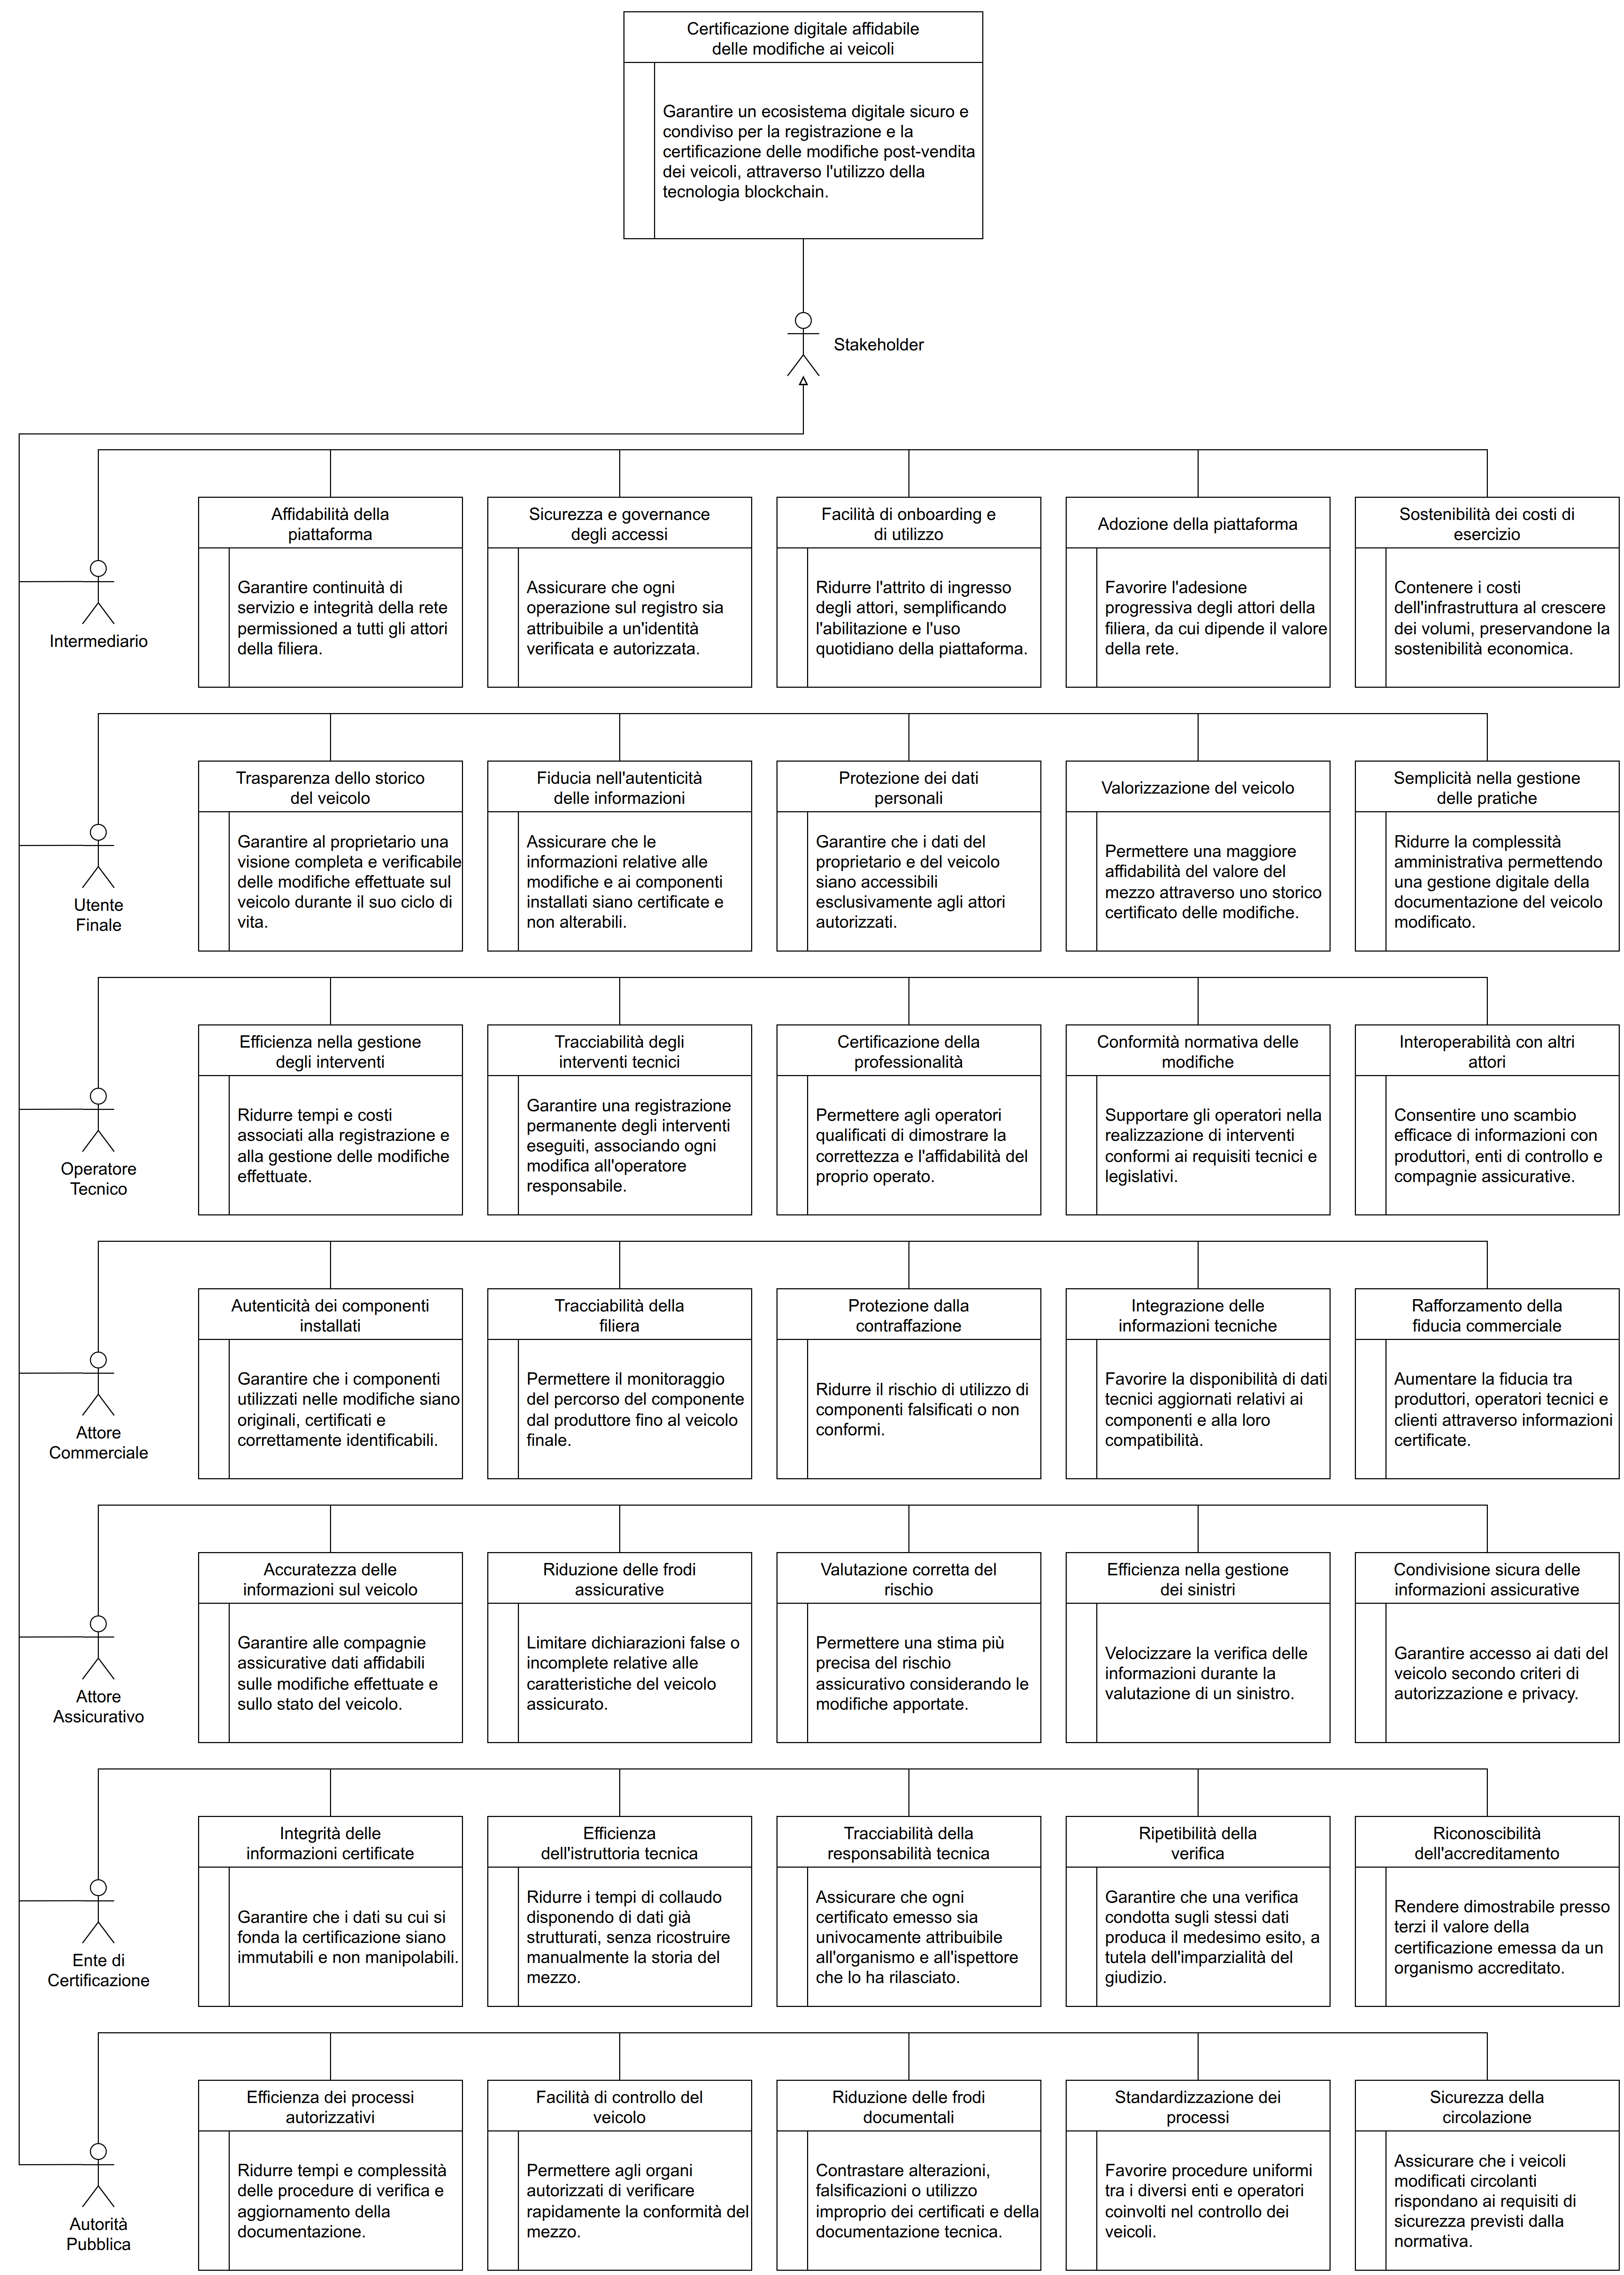
\includegraphics[height=0.85\textheight]{imgs/context/softgoal_diagram.png}}
    \caption{Softgoal Diagram}
    \label{fig:softgoal-diagram}
\end{figure}

\subsubsection*{Softgoal dell'Intermediario}

\begin{itemize}
    \item \textbf{Affidabilit\`a della piattaforma}: garantire continuit\`a di servizio e integrit\`a della rete permissioned a tutti gli attori della filiera.
    \item \textbf{Sicurezza e governance degli accessi}: assicurare che ogni operazione sul registro sia attribuibile a un'identit\`a verificata e autorizzata.
    \item \textbf{Facilit\`a di onboarding e di utilizzo}: ridurre l'attrito di ingresso degli attori, semplificando l'abilitazione e l'uso quotidiano della piattaforma.
    \item \textbf{Adozione della piattaforma}: favorire l'adesione progressiva degli attori della filiera, da cui dipende il valore della rete.
    \item \textbf{Sostenibilit\`a dei costi di esercizio}: contenere i costi dell'infrastruttura al crescere dei volumi, preservandone la sostenibilit\`a economica.
\end{itemize}

\subsubsection*{Softgoal dell'Utente Finale}

\begin{itemize}
    \item \textbf{Trasparenza dello storico del veicolo}: garantire al proprietario una visione completa e verificabile delle modifiche effettuate sul veicolo durante il suo ciclo di vita.
    \item \textbf{Fiducia nell'autenticit\`a delle informazioni}: assicurare che le informazioni relative alle modifiche e ai componenti installati siano certificate e non alterabili.
    \item \textbf{Protezione dei dati personali}: garantire che i dati del proprietario e del veicolo siano accessibili esclusivamente agli attori autorizzati.
    \item \textbf{Valorizzazione del veicolo}: permettere una maggiore affidabilit\`a del valore del mezzo attraverso uno storico certificato delle modifiche.
    \item \textbf{Semplicit\`a nella gestione delle pratiche}: ridurre la complessit\`a amministrativa permettendo una gestione digitale della documentazione del veicolo modificato.
\end{itemize}

\subsubsection*{Softgoal dell'Operatore Tecnico}

\begin{itemize}
    \item \textbf{Efficienza nella gestione degli interventi}: ridurre tempi e costi associati alla registrazione e alla gestione delle modifiche effettuate.
    \item \textbf{Tracciabilit\`a degli interventi tecnici}: garantire una registrazione permanente degli interventi eseguiti, associando ogni modifica all'operatore responsabile.
    \item \textbf{Certificazione della professionalit\`a}: permettere agli operatori qualificati di dimostrare la correttezza e l'affidabilit\`a del proprio operato.
    \item \textbf{Conformit\`a normativa delle modifiche}: supportare gli operatori nella realizzazione di interventi conformi ai requisiti tecnici e legislativi.
    \item \textbf{Interoperabilit\`a con altri attori}: consentire uno scambio efficace di informazioni con produttori, enti di controllo e compagnie assicurative.
\end{itemize}

\subsubsection*{Softgoal dell'Attore Commerciale}

\begin{itemize}
    \item \textbf{Autenticit\`a dei componenti installati}: garantire che i componenti utilizzati nelle modifiche siano originali, certificati e correttamente identificabili.
    \item \textbf{Tracciabilit\`a della filiera}: permettere il monitoraggio del percorso del componente dal produttore fino al veicolo finale.
    \item \textbf{Protezione dalla contraffazione}: ridurre il rischio di utilizzo di componenti falsificati o non conformi.
    \item \textbf{Integrazione delle informazioni tecniche}: favorire la disponibilit\`a di dati tecnici aggiornati relativi ai componenti e alla loro compatibilit\`a.
    \item \textbf{Rafforzamento della fiducia commerciale}: aumentare la fiducia tra produttori, operatori tecnici e clienti attraverso informazioni certificate.
\end{itemize}

\subsubsection*{Softgoal dell'Attore Assicurativo}

\begin{itemize}
    \item \textbf{Accuratezza delle informazioni sul veicolo}: garantire alle compagnie assicurative dati affidabili sulle modifiche effettuate e sullo stato del veicolo.
    \item \textbf{Riduzione delle frodi assicurative}: limitare dichiarazioni false o incomplete relative alle caratteristiche del veicolo assicurato.
    \item \textbf{Valutazione corretta del rischio}: permettere una stima pi\`u precisa del rischio assicurativo considerando le modifiche apportate.
    \item \textbf{Efficienza nella gestione dei sinistri}: velocizzare la verifica delle informazioni durante la valutazione di un sinistro.
    \item \textbf{Condivisione sicura delle informazioni assicurative}: garantire accesso ai dati del veicolo secondo criteri di autorizzazione e privacy.
\end{itemize}

\subsubsection*{Softgoal dell'Ente di Certificazione}

\begin{itemize}
    \item \textbf{Integrit\`a delle informazioni certificate}: garantire che i dati su cui si fonda la certificazione siano immutabili e non manipolabili.
    \item \textbf{Efficienza dell'istruttoria tecnica}: ridurre i tempi di collaudo disponendo di dati gi\`a strutturati, senza ricostruire manualmente la storia del mezzo.
    \item \textbf{Tracciabilit\`a della responsabilit\`a tecnica}: assicurare che ogni certificato emesso sia univocamente attribuibile all'organismo e all'ispettore che lo ha rilasciato.
    \item \textbf{Ripetibilit\`a della verifica}: garantire che una verifica condotta sugli stessi dati produca il medesimo esito, a tutela dell'imparzialit\`a del giudizio.
    \item \textbf{Riconoscibilit\`a dell'accreditamento}: rendere dimostrabile presso terzi il valore della certificazione emessa da un organismo accreditato.
\end{itemize}

\subsubsection*{Softgoal dell'Autorit\`a Pubblica}

\begin{itemize}
    \item \textbf{Efficienza dei processi autorizzativi}: ridurre tempi e complessit\`a delle procedure di verifica e aggiornamento della documentazione.
    \item \textbf{Facilit\`a di controllo del veicolo}: permettere agli organi autorizzati di verificare rapidamente la conformit\`a del mezzo.
    \item \textbf{Riduzione delle frodi documentali}: contrastare alterazioni, falsificazioni o utilizzo improprio dei certificati e della documentazione tecnica.
    \item \textbf{Standardizzazione dei processi}: favorire procedure uniformi tra i diversi enti e operatori coinvolti nel controllo dei veicoli.
    \item \textbf{Sicurezza della circolazione}: assicurare che i veicoli modificati circolanti rispondano ai requisiti di sicurezza previsti dalla normativa.
\end{itemize}

\subsection{Softgoal Dependency Diagram}

Il \textbf{Softgoal Dependency Diagram} riportato in Figura~\ref{fig:softgoal-dependency} sposta l'attenzione dalle singole qualit\`a alla rete di relazioni che intercorre tra di esse. Alle linee continue del diagramma precedente, che associano ciascun softgoal al proprio stakeholder, si affiancano qui frecce tratteggiate che rappresentano le dipendenze reciproche. Esse vanno interpretate come segue:

\begin{itemize}
    \item l'etichetta \textbf{``+'' (contributes)} indica una relazione di rinforzo: il softgoal da cui parte la coda della freccia favorisce la realizzazione del softgoal su cui ricade la testa;
    \item l'etichetta \textbf{``$-$'' (hinders)} indica una relazione di ostacolo: il perseguimento del primo softgoal rende pi\`u difficile il raggiungimento del secondo, evidenziando un \textit{trade-off} progettuale;
    \item le frecce con \textbf{doppia punta} rappresentano relazioni reciproche, nelle quali il rinforzo o l'ostacolo agisce in entrambe le direzioni.
\end{itemize}

\begin{figure}[H]
    \centering
    \makebox[\textwidth][c]{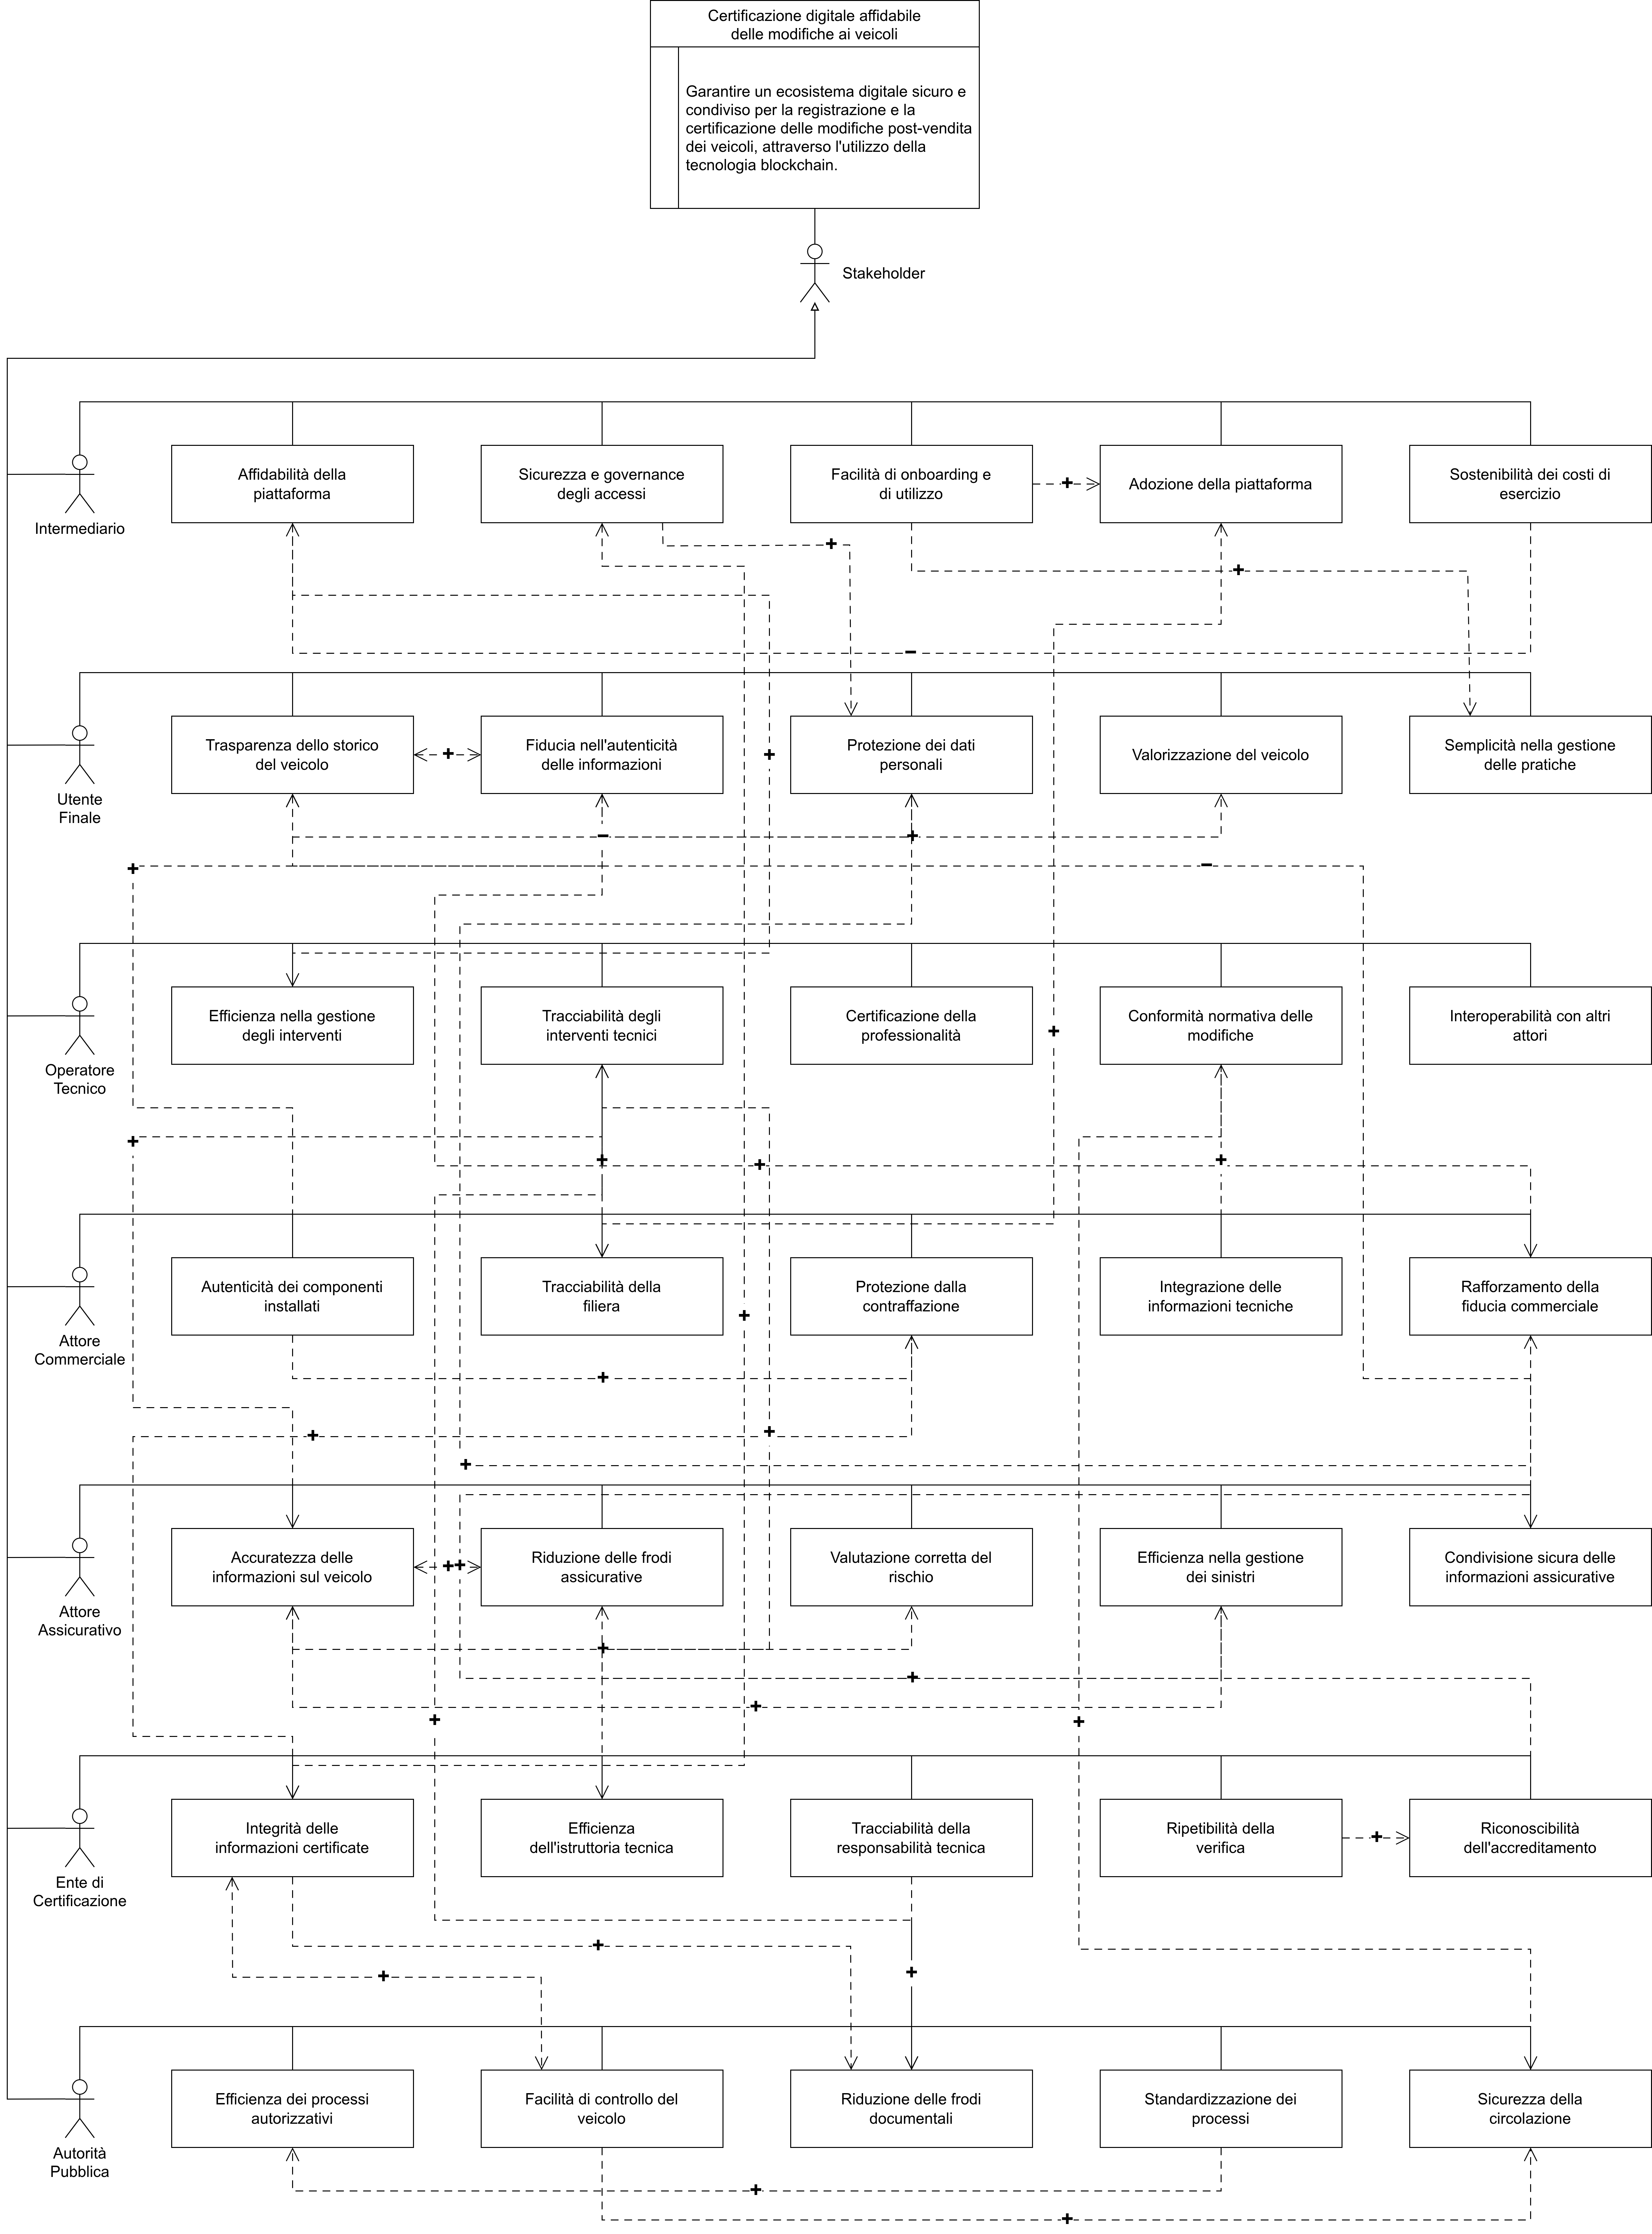
\includegraphics[height=0.85\textheight]{imgs/context/softgoal_dependency.png}}
    \caption{Softgoal Dependency Diagram}
    \label{fig:softgoal-dependency}
\end{figure}

Di seguito vengono analizzate nel dettaglio le singole dipendenze.

\subsubsection*{Contributes (+)}

\begin{itemize}
    \item \textbf{Trasparenza dello storico del veicolo \quad$+$\quad Fiducia nell'autenticit\`a delle informazioni} (reciproca)\\
    Una visione completa e consultabile della storia del mezzo alimenta la fiducia del proprietario nella veridicit\`a di quanto dichiarato; simmetricamente, la certezza che le informazioni non siano alterabili \`e ci\`o che rende la trasparenza effettivamente utile e non meramente formale.

    \item \textbf{Fiducia nell'autenticit\`a delle informazioni \quad$+$\quad Valorizzazione del veicolo} (reciproca)\\
    Il valore di mercato di un veicolo modificato dipende dalla possibilit\`a di dimostrare la regolarit\`a e la qualit\`a degli interventi subiti. Uno storico che gode di credibilit\`a presso gli acquirenti si traduce direttamente in una maggiore affidabilit\`a della stima del mezzo.

    \item \textbf{Autenticit\`a dei componenti installati \quad$+$\quad Fiducia nell'autenticit\`a delle informazioni}\\
    La certezza che i pezzi montati siano originali e correttamente identificati costituisce il presupposto sostanziale della fiducia: un registro accurato di lavorazioni eseguite con componenti non verificati resterebbe formalmente corretto ma privo di valore per il proprietario.

    \item \textbf{Autenticit\`a dei componenti installati \quad$+$\quad Protezione dalla contraffazione}\\
    L'identificazione univoca e certificata di ogni componente rende immediatamente riconoscibile la merce non conforme, riducendo lo spazio di mercato dei ricambi falsificati.

    \item \textbf{Tracciabilit\`a della filiera \quad$+$\quad Tracciabilit\`a degli interventi tecnici} (reciproca)\\
    Conoscere il percorso del componente dal produttore fino al veicolo completa l'informazione sull'intervento eseguito; a sua volta, la registrazione puntuale delle lavorazioni chiude l'ultimo anello della catena di tracciabilit\`a, collegando il pezzo al mezzo su cui \`e stato effettivamente installato.

    \item \textbf{Tracciabilit\`a degli interventi tecnici \quad$+$\quad Accuratezza delle informazioni sul veicolo}\\
    L'associazione permanente di ogni modifica all'operatore responsabile fornisce alle compagnie assicurative dati sullo stato del mezzo la cui provenienza \`e certa e verificabile.

    \item \textbf{Accuratezza delle informazioni sul veicolo \quad$+$\quad Valutazione corretta del rischio} (reciproca)\\
    La stima del rischio assicurativo non pu\`o essere pi\`u precisa dei dati su cui si fonda: disporre di informazioni affidabili sulle modifiche apportate \`e la condizione necessaria per una tariffazione aderente all'effettivo profilo del veicolo.

    \item \textbf{Accuratezza delle informazioni sul veicolo \quad$+$\quad Riduzione delle frodi assicurative} (reciproca)\\
    Quando lo stato del veicolo risulta da un registro non alterabile, lo spazio per dichiarazioni incomplete o mendaci in fase di sottoscrizione si riduce sensibilmente.

    \item \textbf{Riduzione delle frodi assicurative \quad$+$\quad Efficienza nella gestione dei sinistri} (reciproca)\\
    Il venir meno della necessit\`a di accertamenti approfonditi sulla veridicit\`a di quanto dichiarato accorcia i tempi di istruttoria; per converso, una verifica pi\`u rapida e sistematica in sede di sinistro scoraggia i comportamenti opportunistici.

    \item \textbf{Efficienza nella gestione dei sinistri \quad$+$\quad Accuratezza delle informazioni sul veicolo}\\
    La consultazione sistematica del registro in occasione di ogni sinistro alimenta e mantiene aggiornata la base informativa sullo stato effettivo dei veicoli assicurati.

    \item \textbf{Integrit\`a delle informazioni certificate \quad$+$\quad Facilit\`a di controllo del veicolo} (reciproca)\\
    Dati immutabili e non manipolabili consentono agli enti autorizzati di verificare la conformit\`a del mezzo senza dover ricostruire manualmente la documentazione, tanto durante i controlli su strada quanto in sede di revisione periodica.

    \item \textbf{Integrit\`a delle informazioni certificate \quad$+$\quad Riduzione delle frodi documentali}\\
    L'impossibilit\`a tecnica di alterare a posteriori una registrazione elimina alla radice le pratiche di falsificazione e di utilizzo improprio dei certificati di conformit\`a.

    \item \textbf{Integrit\`a delle informazioni certificate \quad$+$\quad Protezione dalla contraffazione} (reciproca)\\
    Il riscontro ufficiale dei dati di omologazione consente di individuare i componenti privi di certificazione valida, rafforzando l'azione di contrasto alla componentistica non conforme; a sua volta, una filiera dei ricambi non contraffatta garantisce che i dati sottoposti a omologazione corrispondano alla reale configurazione del mezzo.

    \item \textbf{Fiducia nell'autenticit\`a delle informazioni \quad$+$\quad Rafforzamento della fiducia commerciale}\\
    La credibilit\`a delle informazioni presso il cliente finale si riflette sull'intera filiera, migliorando il rapporto tra produttori, distributori, operatori tecnici e acquirenti.

    \item \textbf{Integrazione delle informazioni tecniche \quad$+$\quad Conformit\`a normativa delle modifiche}\\
    La disponibilit\`a di dati aggiornati sui componenti e sulla loro compatibilit\`a supporta l'operatore nella progettazione di interventi che rispettino fin dall'origine i requisiti tecnici e legislativi.


    \item \textbf{Protezione dei dati personali \quad$+$\quad Condivisione sicura delle informazioni assicurative} (reciproca)\\
    La definizione di criteri rigorosi di autorizzazione \`e ci\`o che rende praticabile la condivisione dei dati con le compagnie: senza un presidio credibile della riservatezza, l'accesso non sarebbe accettato dai proprietari. Simmetricamente, disciplinare l'accesso assicurativo secondo criteri espliciti rafforza la protezione complessiva dei dati del proprietario.

    \item \textbf{Riduzione delle frodi documentali \quad$+$\quad Tracciabilit\`a degli interventi tecnici} (reciproca)\\
    Il contrasto alla falsificazione documentale valorizza la registrazione puntuale delle lavorazioni, che a sua volta costituisce lo strumento operativo attraverso cui le alterazioni vengono rese rilevabili.

    \item \textbf{Sicurezza e governance degli accessi \quad$+$\quad Protezione dei dati personali}\\
    La verifica delle identit\`a e le politiche di autorizzazione definite dall'Intermediario costituiscono il presidio tecnico su cui si regge la riservatezza dei dati del proprietario: senza un controllo puntuale di chi accede a che cosa, ogni garanzia di privacy resterebbe una dichiarazione di intenti.

    \item \textbf{Sicurezza e governance degli accessi \quad$+$\quad Integrit\`a delle informazioni certificate} (reciproca)\\
    Solo operazioni attribuibili a soggetti verificati producono registrazioni su cui un organismo possa fondare una certificazione; simmetricamente, l'immutabilit\`a del dato certificato \`e ci\`o che rende sensato il presidio sugli accessi.

    \item \textbf{Affidabilit\`a della piattaforma \quad$+$\quad Efficienza nella gestione degli interventi}\\
    Continuit\`a di servizio e prestazioni stabili sono la precondizione perch\'e l'operatore registri le lavorazioni contestualmente all'esecuzione, senza che l'adempimento digitale rallenti il ciclo di lavoro in officina.

    \item \textbf{Facilit\`a di onboarding e di utilizzo \quad$+$\quad Adozione della piattaforma}\\
    Un processo di abilitazione semplice abbassa la soglia di ingresso e accelera l'adesione degli attori alla rete, in particolare delle realt\`a di piccole dimensioni prive di strutture informatiche interne.

    \item \textbf{Facilit\`a di onboarding e di utilizzo \quad$+$\quad Semplicit\`a nella gestione delle pratiche}\\
    Un'interfaccia immediata riduce l'onere amministrativo percepito dal proprietario nella gestione della documentazione del mezzo.

    \item \textbf{Adozione della piattaforma \quad$+$\quad Tracciabilit\`a della filiera} (reciproca)\\
    Il valore di un registro condiviso cresce con il numero di attori che vi partecipano: la tracciabilit\`a dal produttore al veicolo \`e conseguibile solo se tutti gli anelli della catena vi aderiscono e, a sua volta, una filiera effettivamente tracciata rende conveniente l'adesione di chi ancora ne \`e fuori.

    \item \textbf{Tracciabilit\`a degli interventi tecnici \quad$+$\quad Efficienza dell'istruttoria tecnica}\\
    Disporre di lavorazioni gi\`a registrate e attribuite al rispettivo operatore evita all'organismo di certificazione di ricostruire manualmente la storia del mezzo, abbreviando sensibilmente l'istruttoria che precede il collaudo.

    \item \textbf{Ripetibilit\`a della verifica \quad$+$\quad Riconoscibilit\`a dell'accreditamento}\\
    Un giudizio tecnico riproducibile a parit\`a di dati \`e ci\`o che rende credibile, e quindi spendibile presso terzi, l'accreditamento dell'organismo che lo emette.

    \item \textbf{Riconoscibilit\`a dell'accreditamento \quad$+$\quad Rafforzamento della fiducia commerciale}\\
    Il riconoscimento di cui gode l'organismo che certifica si trasferisce sulla reputazione dell'intera filiera che ne utilizza i certificati.

    \item \textbf{Tracciabilit\`a della responsabilit\`a tecnica \quad$+$\quad Riduzione delle frodi documentali}\\
    L'attribuzione univoca di ogni certificato all'organismo e all'ispettore che lo ha emesso rende immediatamente individuabile ogni documento apocrifo o rilasciato da soggetti non abilitati.

    \item \textbf{Standardizzazione dei processi \quad$+$\quad Efficienza dei processi autorizzativi}\\
    Procedure uniformi tra enti diversi eliminano le duplicazioni istruttorie e accorciano i tempi delle autorizzazioni.

    \item \textbf{Facilit\`a di controllo del veicolo \quad$+$\quad Sicurezza della circolazione}\\
    Controlli su strada rapidi e non ambigui aumentano la probabilit\`a di intercettare i veicoli non conformi prima che si traducano in un pericolo per la circolazione.

    \item \textbf{Conformit\`a normativa delle modifiche \quad$+$\quad Sicurezza della circolazione}\\
    Interventi progettati fin dall'origine nel rispetto dei requisiti tecnici e legislativi riducono alla fonte il numero di mezzi irregolari immessi in circolazione.
\end{itemize}

\subsubsection*{Hinders ($-$)}

\begin{itemize}
    \item \textbf{Trasparenza dello storico del veicolo \quad$-$\quad Protezione dei dati personali} (reciproca)\\
    Si tratta del principale \textit{trade-off} del sistema. Ogni ampliamento della visibilit\`a sullo storico del mezzo comporta l'esposizione di informazioni riconducibili al proprietario e alle sue abitudini; per converso, ogni restrizione posta a tutela della riservatezza riduce la completezza dell'informazione effettivamente consultabile. Il conflitto non pu\`o essere risolto a favore di uno dei due obiettivi, ma va governato attraverso politiche di accesso selettivo che differenzino i dati visibili in funzione del ruolo del richiedente.

    \item \textbf{Condivisione sicura delle informazioni assicurative \quad$-$\quad Trasparenza dello storico del veicolo}\\
    I vincoli di autorizzazione e di \textit{privacy} che regolano l'accesso delle compagnie ai dati del veicolo, pur necessari, introducono filtri che limitano la visione complessiva dello storico disponibile agli altri attori, riducendo il grado di trasparenza effettivamente conseguibile.

    \item \textbf{Sostenibilit\`a dei costi di esercizio \quad$-$\quad Affidabilit\`a della piattaforma}\\
    Il contenimento dei costi dell'infrastruttura comprime i margini di ridondanza e di capacit\`a con cui si garantisce la continuit\`a del servizio. \`E il \textit{trade-off} tipico di un'infrastruttura distribuita e ricade interamente sull'Intermediario, che deve individuare il punto di equilibrio tra livello di servizio offerto e costo per transazione registrata.
\end{itemize}

Nel complesso, la rete di dipendenze evidenzia come le qualit\`a attese dai diversi stakeholder siano largamente convergenti: la quasi totalit\`a delle relazioni \`e di tipo \textit{contributes}, a conferma del fatto che un registro condiviso e non alterabile produce benefici simultanei lungo tutta la filiera. Le tre relazioni di ostacolo individuate segnalano altrettanti vincoli progettuali. Le prime due ruotano attorno alla tensione tra apertura informativa e riservatezza, che si conferma il \textit{trade-off} pi\`u delicato da governare nelle fasi successive di definizione dell'architettura e delle politiche di accesso; la terza riguarda l'Intermediario e contrappone il livello di servizio garantito al costo dell'infrastruttura che lo sostiene, questione che sar\`a ripresa nel Capitolo~7 in sede di valutazione economica.
